%! TeX program = lualatex
\documentclass[a4paper,11pt]{article} 
% packages
\usepackage{fontspec}
\setmainfont{EB Garamond}
% for tironian et fallback
% % \directlua{luaotfload.add_fallback
% % ("emojifallback",
% %      {"Noto Serif:mode=harf"}
% % )}
% % \setmainfont{EB Garamond}[RawFeature={fallback=emojifallback}]

\setmonofont[Scale=MatchLowercase]{Deja Vu Sans Mono}
\usepackage[a4paper,left=2cm,right=2cm,top=\dimexpr15mm+1.5\baselineskip,bottom=2cm]{geometry}
\setlength{\parindent}{0pt}

\usepackage{fancyhdr}       % Headers and footers 
\fancyhead[R]{\normalfont \leftmark}
\fancyhead[L]{}
\pagestyle{fancy}

\usepackage{microtype}      % Slightly tweak font spacing for aesthetics
\usepackage[english]{babel} % Language hyphenation and typographical rules
\usepackage[final, colorlinks = true, urlcolor = blue, linkcolor = black]{hyperref} 
\usepackage{changepage}     % adjust margins on the fly
\usepackage{amsmath}

\usepackage{minted}
\usemintedstyle{algol_nu}
\usepackage{xcolor}
\usepackage{algpseudocode}

\usepackage{tkz-graph}
\usetikzlibrary{positioning, fit, shapes.geometric}
\usepackage{pgfplots}
\pgfplotsset{width=\textwidth,compat=1.9}

\usepackage{caption}
\newenvironment{code}{\captionsetup{type=listing}}{}

\usepackage[yyyymmdd]{datetime}
\renewcommand{\dateseparator}{-}

\usepackage{titlesec}

\begin{document}
\begin{titlepage}
    \begin{center}
        \hrule
        \vspace*{0.6cm}
        \huge \textbf{CT3532}
        \vspace*{0.6cm}
        \hrule
        \LARGE
       \vspace{0.5cm}
        DATABASE SYSTEMS II
       \vspace{0.5cm}
       \hrule
            
       \vfill
       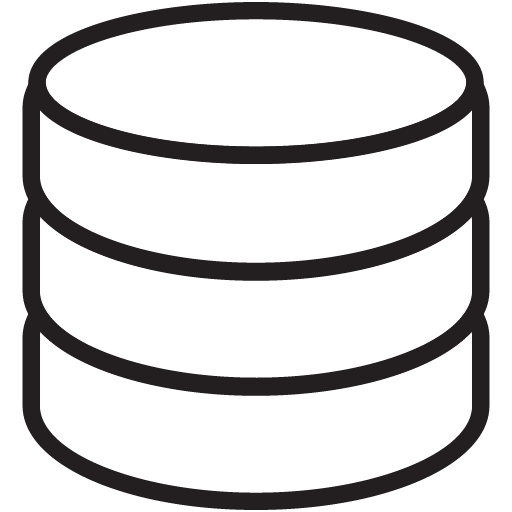
\includegraphics[width=0.7\textwidth]{images/db.png}
        \vfill

        \Large
       \vspace{0.5cm}
       \hrule
       \vspace{0.5cm}
       \textbf{Andreas Ó hAoḋa}
       % \vspace{0.5cm}
       % \hrule
       % \vspace{0.5cm}
            
       \normalsize
       University of Galway

       \today

       \vspace{0.5cm}
       \hrule
    \end{center}
\end{titlepage}

\pagenumbering{roman}
\newpage
\tableofcontents
\newpage
\setcounter{page}{1}
\pagenumbering{arabic}

\section{Introduction}
\subsection{Recommended Texts}
\begin{itemize}
    \item   \emph{Fundamentals of Database Systems} by Elmasri and Navathe 005.74 ELM
    \item   \emph{Database system concepts} by Silberschatz, A. 005.74 SIL
\end{itemize}

\subsection{Assessment}
Continuous Assessment accounts for 30\% of the final grade, and the exam accounts for the remaining 70\%.
Plagiarism of assignments is not permitted - This is strictly enforced.

\subsubsection{Assignments}

\section{Design}
\subsection{Re-cap}
\textbf{Normalisation} can be used to develop a normalised relational schema given the universal relation, and verify 
the correctness of relational schema developed from conceptual design.
We decompose relations such that it satisfies successively restrictive normal forms.
\\\\
Desirable properties of a relational schema include:
\begin{itemize}
    \item   \textbf{Clear semantics of a relation:} The \textbf{semantics} of a relation refers to how the attributes
            grouped together in a relation are to be interpreted. 
            If ER modelling is done carefully and the mapping  is undertaken correctly, it is likely that the semantics of 
            the resulting relation will be \emph{clear}.
            One should try to design a relation so that it is easy to explain its meaning.
    \item   \textbf{Reducing the number of redundant values in tuples:} The presence of redundancy leads to waste of
            storage space and potential for anomalies (deletion, update, insertion).
            One should try to design relations so that no anomalies may occur. If an anomaly can occur, it should be noted.
            Normalisation will remove many of the potential anomalies.
    \item   \textbf{Reducing the number of null values in tuples:} Having null values is often necessary, but it can
            create problems, such as:
            \begin{itemize}
                \item   Wasted space. 
                \item   Different interpretations, i.e.: attribute does not apply to this tuple, attribute value is 
                        unknown, attribute value is known but absent, etc.
            \end{itemize}

    \item   \textbf{Disallowing the possibility of generating spurious tuples:} If a relation $R$ is decomposed into $R_1$
            \& $R_2$ and connected via a primary key -- foreign key pair, then performing an equi-join between $R_1$ \&
            $R_2$ on the involved keys should not produce tuples that were not in the original relation $R$.
\end{itemize}

More formally, we typically have a relation $R$ and a set of functional dependencies $F$, defined over $R$. 
We wish to create a decomposition $D = \{R_1, R_2, \dots, R_n\}$
We wish to guarantee certain properties of this decomposition.
We require that all attributes in the original $R$ be maintained in the decomposition, \textit{id est}:
$R = R_1 \cup R_2 \cup \dots \cup R_n$
\begin{itemize}
    \item   A relation is said to be in the \textbf{First Normal Form (1NF)} if there are no repeating fields. 
    \item   A relation is said to be in the \textbf{Second Normal Form (2NF)} if it is in 1NF and if every non-prime 
            attribute is fully functionally dependent on the key.
    \item   A relation is said to be in the \textbf{Third Normal Form (3NF)} if it is in 2NF and if no non-prime 
            attribute is transitively dependent on the key.
    \item   A relation is said to be in the \textbf{Boyce-Codd Normal Form (BCNF)} if the relation is in 3NF and if 
            every determinant is a candidate key.
\end{itemize}

\subsubsection{Example}
\begin{table}[H]
    \centering
    \begin{tabular}{lll}
    \hline
    StudentNo & Major & Advisor   \\ \hline
    123       & I.T.  & Smith     \\
    123       & Econ  & Murphy    \\
    444       & Biol. & O' Reilly \\
    617       & I.T.  & Jones     \\
    829       & I.T.  & Smith     \\ \hline
    \end{tabular}
    \caption{Sample Data}
\end{table}

Constraints:
\begin{itemize}
    \item   A student may have more than one major. 
    \item   For each major, a student can have only one advisor. 
    \item   Each major can have several advisors. 
    \item   Each advisor advises one major.
    \item   Each advisor can advise several students.
\end{itemize}

Functional dependencies:
\begin{itemize}
    \item   \{StudentNo, Major\} {\rightarrow} \{Advisor\}
    \item   \{Advisor\} {\rightarrow} \{Major\}
\end{itemize}

An update anomaly may exist: If student 44 changes major, we lose information that O' Reilly supervises Biology.
To solve this, we can decompose the tables so as to satisfy BCNF: 
\begin{itemize}
    \item   TAKES: \underline{StudentNo, Advisor}
    \item   ADVISES: \underline{Advisor}, Major
\end{itemize}

\subsubsection{General Rule}
Consider a relation $R$ with functional dependencies $F$. 
If $X \rightarrow Y$ violates BCNF, decompose $R$ into:
\begin{itemize}
    \item   $\{R - Y\}$
    \item   $\{XY\}$
\end{itemize}

\subsubsection{Exercise}
Let $R = \{A, B, C, D, E, F, G, H\}$.
The functional dependencies defined over $R$ are:
\begin{itemize}
    \item   $A \rightarrow D$
    \item   $B \rightarrow E$
    \item   $E \rightarrow F$
    \item   $F \rightarrow G$
    \item   $F \rightarrow H$
    \item   $\{A, B\} \rightarrow C$
    \item   $C \rightarrow A$
\end{itemize}


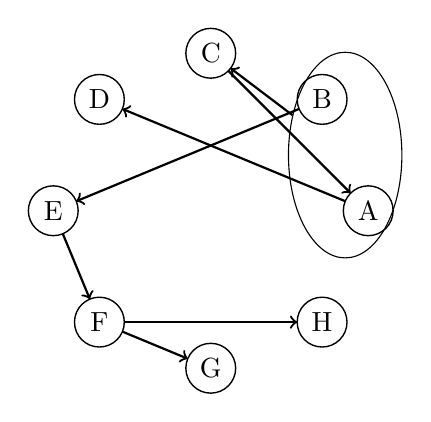
\begin{tikzpicture}
\SetGraphUnit{2}
\SetUpEdge[style={->}]
\Vertices{circle}{A, B, C, D, E, F, G, H}
\node[ellipse, draw=black, fit=(A) (B), inner sep=-1mm] (AB) {};

\Edge(A)(D)
\Edge(B)(E)
\Edge(E)(F)
\Edge(F)(G)
\Edge(F)(H)
\Edge(AB)(C)
\Edge(C)(A)
\end{tikzpicture}


Decompose $R$ such that the BCNF is satisfied.


\section{Design by Synthesis}
\subsection{Background}
Typically, we have the relation $R$ and a set of functional dependencies $F$. 
We wish to create a decomposition $D = R_1, R_2, \dots, R_m$. 
Clearly, all attributes of $R$ must occur in at least one schema $R_i$, \textit{id est}: $U^{m}_{i=1} R_i = R$. 
This is known as the \textbf{attribute preservation} constraint.
\\\\ 
A \textbf{functional dependency} is a constraint between two sets of attributes. 
A functional dependency $X \rightarrow Y$ exists for all tuples $t_1$ \& $t_2$ if $t_1[X] = t_2[X]$, then $t_2$ if
$t_1[Y] = t_2[Y]$.
We usually only specify the obvious functional dependencies, there may be many more.
Given a set of functional dependencies $F$, the \textbf{closure of \textit{F}}, denoted $F^+$, refers to all dependencies that
can be derived from $F$.

\subsubsection{Armstrong's Axioms}
\textbf{Armstrong's Axioms} are a set of inference rules that allow us to deduce all functional dependencies from a given 
initial set.
They are:
\begin{itemize}
    \item   \textbf{Reflexivity:} if $X \supseteq Y$, then $X \rightarrow Y$. 
    \item   \textbf{Augmentation:} if $X \rightarrow Y$, then $XZ \rightarrow YZ$.
    \item   \textbf{Transitivity:} if $X \rightarrow Y$, $Y \rightarrow Z$, then $X \rightarrow Z$. 
    \item   \textbf{Projectivity:} if $X \rightarrow YZ$, then $X \rightarrow Z$. 
    \item   \textbf{Additivity:} if $X \rightarrow Y$, $X \rightarrow Z$, then $X \rightarrow YZ$. 
    \item   \textbf{Pseudo-transitivity:} if $X \rightarrow Y$, $WY \rightarrow Z$, then $WX \rightarrow Z$. 
\end{itemize}

The first three rules have been shown to be \textbf{sound} \& \textbf{complete}:
\begin{itemize}
    \item   \textbf{Sound:} Given a set $F$ on a relation $R$, any dependency we can infer from $F$ using the first three 
            rules holds for every state of $r$ of $R$ that satisfies the dependencies in $F$.
    \item   \textbf{Complete:} We can use the first three rules repeatedly to infer all possible dependencies that can be 
            inferred from $F$.
\end{itemize}

For any sets of attributes $A$, we can infer $A^+$, the set of attributes that are functionally determined by $A$ given 
a set of functional dependencies.

% skipped page 8 here
\subsubsection{Cover Sets}
A set of functional dependencies $F$, \textbf{covers} a set of functional dependencies $E$ if every functional dependency
in $E$ is in $F^+$.
\\\\ 
Two sets of functional dependencies $E$ \& $F$ are equivalent if $E^+ = F^+$.
We can check if $F$ covers $E$ by calculating $A^+$ with respect to $F$ for each functional dependency $A \rightarrow B$ 
and then checking that $A^+$ includes all the attributes of $B$.
\\\\ 
A set of functional dependencies, $F$< is \textbf{minimal} if: 
\begin{itemize}
    \item   Every functional dependency in $F$ has a single attribute for its right-hand side. 
    \item   We cannot remove any dependency from $F$ and maintain a set of dependencies equivalent to $F$. 
    \item   We cannot replace any dependency $X \rightarrow A$ with a dependency $Y \rightarrow A$ where $Y \subset X$, 
            and still maintain a set of dependencies equivalent to $F$.
\end{itemize}

All functional dependencies $X \rightarrow Y$ specified in $F$ should exist in one of the schema $R_i$, or should be 
inferable from the dependencies in $R_i$; this is known as the \textbf{dependency preservation} constraint.
Each functional dependency specifies some constraint; if the dependency is absent, then some desired constraint is also 
absent.
If a functional dependency is absent, then we must enforce the constraint in some other manner; this can be inefficient.
\\\\ 
Given $F$ \& $R$, the \textbf{projection} of $F$ on $R_i$, denoted $\pi_{R_i}(F)$ where $R_i$ is a subset of $R$, is the 
set $X \rightarrow Y$ in $F^+$ such that attributes $X \cup Y \in R_i$.
A decomposition of $R$ is dependency-preserving if:
$$
((\pi_{R_1}(F)) \cup \dots \cup (\pi_{R_m}(F)))^+ = F^+
$$

\textbf{Theorem:}
It is always possible to find a decomposition $D$ with respect to $F$ such that: 
\begin{enumerate}
    \item   The decomposition is dependency-preserving.
    \item   All $R_i$ in $D$ are in 3NF.
\end{enumerate}

We can always guarantee a dependency-preserving decomposition to 3NF. 
\textbf{Algorithm:}
\begin{enumerate}
    \item   Find a minimal cover set $G$ for $F$.
    \item   For each left-hand side $X$ of a functional dependency in $G$, create a relation
            $X \cup A_1 \cup A_2 \dots A_m$ in $D$, where $X \rightarrow A_1$, $X \rightarrow A_2, \dots$ are the only 
            dependencies in $G$ with $X$ as a left-hand side.
    \item   Group any remaining attributes into a single relation.
\end{enumerate}

\subsubsection{Lossless Joins}
Consider the following relation:
\begin{itemize}
    \item   EMPPROJ: \underline{ssn, pnumber}, hours, ename, pname, plocation
\end{itemize}
and its decomposition to:
\begin{itemize}
    \item   EMPPROJ1: \underline{ename, plocation}
    \item   EMPLOCAN: \underline{ssn, pno}, hrs, pname, plocation
\end{itemize}
If we perform a natural join on these relations, we may generate spurious tuples.
When a natural join is issued against relations, no spurious tuples should be generated.
A decomposition $D = \{R_1, R_2, \dots R_n\}$ of $R$ has the \textbf{lossless join} (or non-additive join) property with
regards to $F$ on $R$ if every instance $r$ of the following holds:
$$ \bowtie (\pi_{R_1}(r), \dots \pi_{R_m}(r)) = r $$
We can automate a procedure for testing for the lossless property. 
We can also automate the decomposition of $R$ into $R_1, \dots R_m$ such that is possesses the lossless join property.
\\\\

A decomposition $D = \{R_1, R_2\}$ has the lossless property if \& only if:
\begin{itemize}
    \item   The functional dependency $(R_1 \cap R_2) \rightarrow \{R_1 - R_2\}$ is in $F^+$, \emph{or}
    \item   The functional dependency $(R_1 \cap R_2) \rightarrow \{R_2 - R_1\}$ is in $F^+$.
\end{itemize}

Furthermore, if a decomposition has the lossless property and we decompose one of $R_i$ such that this also is a lossless 
decomposition, then replacing that decomposition of $R_i$ in the original decomposition will result in a lossless 
decomposition.
\\\\ 
\textbf{Algorithm:} To decompose to BCNF:
\begin{enumerate}
    \item   Let $D = R$.
    \item   While there is a schema $B$ in $D$ that violates BCNF, do:
            \begin{enumerate}
                \item   Find the functional dependency $(X \rightarrow Y)$ that violates BCNF.
                \item   Replace $B$ with $(B-Y)$ \& $(X \cup Y)$.
            \end{enumerate}
\end{enumerate}

This guarantees a decomposition such that all attributes are preserved, the lossless join property is enforced, 
and all $R_i$ are in BCNF.
It is not always possible to decompose $R$ into a set of $R_i$ such that all $R_i$ satisfy BCNF and properties 
of lossless joins \& dependency preservation are maintained.
We can guarantee a decomposition such that:
\begin{itemize}
    \item   All attributes are preserved.
    \item   All relations are in 3NF.
    \item   All functional dependencies are maintained. 
    \item   The lossless join property is maintained.
\end{itemize}

\textbf{Algorithm:} Finding a key for a relation schema $R$.
\begin{enumerate}
    \item   Set $K := R$.
    \item   For each attribute $A \in K$, compute $(K-A)^+$ with respect to the set of functional dependencies.
            If $(K-A)^+$ contains all the attributes in $R$, the set $K := K - \{A\}$.
\end{enumerate}

Given a set of functional dependencies $F$, we can develop a minimal cover set. 
Using this, we can decompose $R$ into a set of relations such that all attributes are preserved, all functional 
dependencies are preserved, the decomposition has the lossless join property, and all relations are in 3NF.
The advantages of this are that it provides a good database design and can be automated.
The primary disadvantage is that often, numerous good designs are possible.

\section{B Trees \& B+ Trees}
\subsection{Generalised Search Tree}
In a \textbf{Generalised Search Tree}, each node has the format $P_1, K_1, P_2, K_2, \dots, P_{n-1}, K_{n-1}, P_n$ 
where $P_i$ is a \textbf{tree value} and $K_i$ is a \textbf{search value}.
Hence, the number of values per node depends on the size of the key field, block size, \& block pointer size.
The following constraints hold:
\begin{itemize}
    \item   $K_1 < K_2 < \dots < K_{n-1} < K_n$.
    \item   For all values $x$ in a sub-tree pointed to $P_i$, $K_{i-1} < x < K_i$.
    \item   The number of tree pointers per node is known as the \textbf{order} or $\rho$ of the tree.
\end{itemize}

\subsubsection{Efficiency}
For a generalised search tree: $T(N) = O(\text{log}(N))$, assuming a balanced tree. 
In order to guarantee this efficiency in searching \& other operations, we need techniques to ensure that the tree is
always balanced.

\subsection{B Trees}
A \textbf{B tree} is a balanced generalised search tree.
B trees can be viewed as a dynamic multi-level index. 
The properties of a search tree still hold and the algorithms for insertion \& deletion of values are modified in order.
The node structure contains a record pointer for each key value.
The node structure is as follows:
$$
P_1 < K_1, Pr_1 > P_2 < K_2, Pr2 > \dots P_{n-1} < K_{n-1}, Pr_{n-1} > P_n
$$

\subsubsection{Example}
Consider a B Tree of order 3 (two values and three tree pointers per node/block).
Insert records with key values: 10, 6, 8, 14, 4, 16, 19, 11, 21.

\subsubsection{Algorithm to Insert a Value into a B Tree}
\begin{enumerate}
    \item   Find the appropriate leaf-level node to insert a value.
    \item   If space remains in the leaf-level node, then insert the new value in the correct location.
    \item   If no space remains, we need to deal with collisions.
\end{enumerate}

\subsubsection{Dealing with Collisions}
\begin{enumerate}
    \item   Split node into left \& right nodes.
    \item   Propagate the middle value up a level and place its value in a node there. Note that this propagation may 
            cause further propagations and even the creation of a new root node.
    \item   Place the values less than the middle value in the left node.
    \item   Place the values greater than the middle value in the right node.
\end{enumerate}

This maintains the balanced nature of the tree, and $O(\text{log}_\rho(N))$ for search, insertion, \& deletion.
However, there is always potential for unused space in the tree. 
Empirical analysis has shown that B trees remain 69\% full given random insertions \& deletions.

\subsubsection{Exercise}
Can you define an algorithm for deletion (at a high level)?
How much work is needed in the various cases (best, average, worst)?

\subsection{B+ Trees}
The most commonly used index type is the \textbf{B+ tree} -- a dynamic, multi-level index. 
B+ trees differ from B trees in terms of structure, and have slightly more complicated insertion \& deletion algorithms.
B+ trees offer increased efficiency over a B Tree and ensures a higher order \rho.

\subsubsection{Node Structure}
B+ trees have two different node structures: internal nodes \& leaf-level nodes.
The internal node structure is:
$$P_1, K_1, P_2, K_2, \dots P_{n-1}, K_{n-1}, P_n$$
All record pointers are maintained at the leaf level in a B+ tree.
There are no record pointers in the internal nodes.
B+ trees have less information per record and hence more search values per node.
\\\\
One tree pointer is maintained at each leaf-level node, which points to the next leaf-level node.
Note that there is only one tree pointer per node at the leaf level.
Each leaf-level node's structure is:
$$K_1, Pr_1, K_2, PR_2, \dots K_m, Pr_m, P_{\text{next}}$$

\subsubsection{Example}
Let $B = 512$, $P = 6$, $K = 10$. 
Assume 30,000 records as before. 
Assume that the tree is 69\% full. 
How many blocks will the tree require? 
How many block accesses will a search require?

\subsubsection{Example}
A tree of order $\rho$ has at most $\rho - 1$ search values per node. 
For a B+ tree, there are two types of tree nodes; hence there are two different orders: $\rho$ \& $\rho_{\text{leaf}}$.
To calculate $\rho_{\text{leaf}}$: 
$$ |P| + (\rho_{\text{leaf}})(|K| + |Pr|) \leq B $$
$$ \rightarrow 17(\rho_{\text{leaf}}) \leq 506 $$
$$ \rho_{\text{leaf}} = 29 $$

Given a fill factor of 69\%:
\begin{itemize}
    \item   Each internal node will have, on average, 22 pointers.
    \item   Each leaf-level node will have, on average, 20 pointers.
\end{itemize}

\begin{itemize}
    \item   Root: 1 node, 21 entries, 22 pointers.
    \item   Level 1: 22 nodes, 462 entries, 484 pointers.
    \item   Level 2: 484 nodes, \dots, etc.
    \item   Leaf Level: \dots
\end{itemize}

Hence, 4 levels are sufficient. 
The number of block accesses $= 4 + 1$.
The number of blocks is $1 + 22 + 484 + \dots$

\section{Hash Tables}
\subsection{Introduction}
Can we improve upon logarithmic searching?
\textbf{Hashing} is a technique that attempts to provide constant time for searching \& insertion, i.e. $O(K)$. 
The basic idea for searching \& insertion is to apply a hash function to the search field of the record;
the return value of the hash function is used to reference a location in the hash table.
\\\\
Care should be taken in designing a hash function.
We usually require a \textbf{fair} hash function.
This is difficult to guarantee if there is no or limited information available about the type of data to be 
stored.
Often, heuristics can be used if domain knowledge is available.
We can have both internal (i.e., some data structure in memory) or external hashing (i.e., to file locations).
We must consider the size of the original table or file.

\subsection{Approaches}
\begin{enumerate}
    \item   Create a hash table containing $N$ addressable ``slots'' which each can contain one record.
    \item   Create a hash function that returns a value to be used in insertion \& searching.
            The value returned by the hash function must be in the correct range, i.e. the address space of the
            hash table
\end{enumerate}

If the range of the keys is that of the address space of the table, we can guarantee constant-time lookup.
However, this is usually not the case as the address space of the table is much smaller than that of the search field.
\\\\
With numeric keys, we can use modulo-division or truncation for hashing.
With character keys, we must first convert to an integer value: this can be achieved by multiplying the ASCII 
code of the characters together and then applying modulo-division.
However, we cannot guarantee constant-time performance as collisions will occur, i.e. two records with different search
values being hashed to the same location in the table; we require a collision resolution policy.
Efficiency then will depend on the number of collisions. 
The number of collisions depends primarily on the load factor $\lambda$ of the file: 
$$
\lambda =  \frac{\text{Number of records}}{\text{Number of slots}}
$$

\subsubsection{Collision Resolution Policies}
\begin{itemize}
    \item   \textbf{Chaining:} if a location is full, add the item to a linked list. 
            Performance degrades if the load factor is high.
            The lookup time is on average $1 + \lambda$.
    \item   \textbf{Linear probing:} if a location is full, then check in a linear manner for the next free space. 
            This can degrade to a linear scan. 
            The performance, if successful is $0.5(1 + \frac{1}{1-\lambda})$ and if unsuccessful is
            $0.5 + (1 + \frac{1}{1 + \lambda}^2)$.
            One big disadvantage of this approach is that it leads to the formation of clusters.
    \item   \textbf{Quadratic probing:} if a location is full, check the location $x + 1$, location $x + 4$, 
            location $(x + n)^2$.
            This results in less clustering.
    \item   \textbf{Double hashing:} if location $x$ is occupied, then apply a second hash function. 
            This can help guarantee an even distribution (a fairer hash function).
\end{itemize}

\subsection{Dynamic Hashing}
The cases that we've considered thus far deal with the idea of a \textbf{fixed hash table}: this is referred to 
as \textbf{static hashing}.
Problems arise if the database grows larger than planned: too many overflow buckets and performance degrades.
A more suitable approach is \textbf{dynamic hashing}, wherein the table or file can be re-sized as needed.

\subsubsection{General Approach}
\begin{enumerate}
    \item   Use a family of hash functions $h_0$, $h_1$, $h_2$, etc.
            $h_{i+1}$ is a refinement of $h_i$.
            E.g., $K \text{mod} 2^i$.
    \item   Develop a base hash function that maps the key to a positive integer.
    \item   Use $h_0(x) = x \text{mod} 2^b$ for a chosen $b$. 
            There will be $2^b$ buckets initially. 
            We can effectively double the size of the table by incrementing $b$.
\end{enumerate}

We only double the number of buckets when re-organising conceptually; we do not actually double the number of 
buckets in practice as it may not be needed.

\subsection{Dynamic Hashing Approaches}
Common dynamic hashing approaches include extendible hashing \& linear hashing.
\textbf{Extendible hashing} involves re-organising the buckets when \& where needed, whereas
\textbf{linear hashing} involves re-organising buckets when but not where needed.

\subsubsection{Extendible Hashing}
\begin{itemize}
    \item   When a bucket overflows, split that bucket in two. A directory is used to achieve this conceptual
            doubling.
    \item   If a collision or overflow occurs, we don't re-organise the file by doubling the number of buckets, 
            as this would be too expensive.
            Instead, we maintain a directory of pointers to buckets, we can effectively double the number of 
            buckets by doubling the directory, splitting just the bucket that overflowed.
            Doubling the directory is much cheaper than doubling the file, as the directory is much smaller than
            the file,
    \item   On overflow, we split the bucket by allocating a new bucket and redistributing its contents.
            We double the directory size if necessary.
\end{itemize}

We maintain a \textbf{local depth} for each bucket, effectively the number of bits needed to hash an item here.
We also maintain a \textbf{global depth} for the directory which is the number of bits used in indexing items.
We can use these values to determine when to split the directory.
\begin{itemize}
    \item   If overflow occurs in a bucket where the local depth = global depth, then split the bucket, 
            redistribute its contents, and double the directory.
    \item   If overflow occurs in a bucket where the local depth < global depth, then split the bucket,
            redistribute its contents, and increase the local depth.
\end{itemize}

If the directory can fit in the memory, then the retrieval for point queries can be achieved with one disk read.

\subsection{Linear Hashing}
\textbf{Linear hashing} is another approach to indexing to a dynamic file.
It is similar to dynamic hashing in that a family of hash functions are used ($h = K \text{mod} 2^i$), but
differs in that no index is needed.
Initially, we create a file of $M$ buckets; $K \text{mod} M^1$ is a suitable hash function.
We will use a family of such functions $K \text{mod} (2^i \times M), i = 0$ initially.
We can view the hashing as comprising of a sequence of phases: for phase $j$, the hash functions
$K \text{mod} 2^i \times M$ \& $K \text{mod} 2^{j+1} \times M$ are used.
\\\\
We \textbf{split a bucket} by redistributing the records into two buckets: the original one \& a new one.
In phase $j$, to determine which ones go into the original while the others go into the new one, we use 
$H_{j+1}(K) = K \text{mod} 2^{j+1} \times M$ to calculate their address.
Irrespective of the bucket which causes the overflow, we always split the next bucket in a \textbf{linear order}.
We begin with bucket 0, and keep track of which bucket to split next $p$.
At the end of a phase when $p$ is equal to the number of buckets present at the start of the phrase, we reset $p$
and a new phase begins ($j$ is incremented).

\section{Joins}
Many approaches \& algorithms can be used to do \textbf{joins}.

\subsection{Nested Loop Join}
To perform the join $r \bowtie s$:
\begin{minted}[texcl, mathescape, linenos, breaklines, frame=single]{text}
for each tuple t_r in r do:
    for each tuple t_s in s do:
        if t_r and t_ satisfy join condition:
            add(t_r, t_s) to result
    end 
end
\end{minted}

This is an expensive approach; every pair of tuples is checked to see if they satisfy the join condition.
If one of the relations fits in memory, it is beneficial to use this in the inner loop (known as the
\textbf{inner relation}).

\subsection{Block nested Loop Join}
The \textbf{block nested loop join} is a variation on the nested loop join that increases efficiency by 
reducing the number of block accesses.
\begin{minted}[texcl, mathescape, linenos, breaklines, frame=single]{text}
for each block B_r in r do:
    for each block B_s in s do:
        for each tuple t_r in B_r do:
            for each tuple t_s in B_s do:
                if t_r and t_s satisfy join condition:
                    add (t_r, t_s) to result
            end
        end
    end
end
\end{minted}

\subsection{Indexed Nested Loop Join}
If there is an index available for the inner table in a nested loop join, we can replace file scans with index 
accesses.

\subsection{Merge Join}
If both relations are sorted on the joining attribute, then we can merge the relations. 
The technique is identical to merging two sorted lists (such as in the ``merge''' step of a Merge-Sort algorithm).
Merge joins are much more efficient than a nested join.
They can also be computed for relations that are not ordered on a joining attribute, but have indexes on the joining 
attribute.

\subsection{Hash Joins}
\begin{enumerate}
    \item   Create a hashing function which maps the join attribute(s) to partitions in a range $1 .. N$. 
    \item   For all tuples in $r$, hash the tuples to $H_{ri}$.
    \item   For all tuples in $s$, hash the tuples to $H_{si}$.
    \item   For $i = 1$ to $N$, join the partitions $H_{ri} = H_{si}$.
\end{enumerate}

\section{Sorting}
Sorting is a very important operation because it is used if a query specifies \mintinline{SQL}{ORDER BY} and is 
used prior to relational operators (e.g. Join) to allow more efficient processing of the operation.
We can sort a relation in two ways:
\begin{itemize}
    \item   \textbf{Physically:} actual order of tuples re-arranged on the disk.
    \item   \textbf{Logically:} build an index and sort index entries.
\end{itemize}

When the relation to be sorted fits in the memory, we can use standard sorting techniques (such as Quicksort).
However, when the relation doesn't fit in memory, we have to use other approaches such as the \textbf{external 
sort merge}, which is essentially an $N$-way merge, an extension of the idea in the merge step of the merge sort 
algorithm.

\begin{minted}[texcl, mathescape, linenos, breaklines, frame=single]{text}
i := 0;
M = number of page frames in main memory buffer

repeat 
    read M blocks of the relation 
    sort M blocks in memory
    write sorted data to file R_i
until end of relation 

read first block of each R_i into memory
repeat 
    choose first (in sort order) from pages
    write tuple to output
    remove tuple from buffer
    if any buffer R_i empty and not eof(R_i)
        read next block from R_i into memory
    until all pages empty
\end{minted}

\section{Parallel Databases}
Characteristics of \textbf{Parallel databases} include:
\begin{itemize}
    \item   Increased transaction requirements.
    \item   Increased volumes of data, particularly in data-warehousing.
    \item   Many queries lend themselves easily to parallel execution.
    \item   Can reduce the time required to retrieve relations from disk by partitioning relations onto a set of 
            disks.
    \item   Horizontal partitioning is usually used.
            Subsets of a relation are sent to different disks.
\end{itemize}

\subsection{Query Types}
Common types of queries include:
\begin{itemize}
    \item   \textbf{Batch processing:} scanning an entire relation.
    \item   \textbf{Point-Queries:} return all tuples that match some value.
    \item   \textbf{Range-Queries:} return all tuples with some value in some range.
\end{itemize}

\subsection{Partitioning Approaches}
\subsubsection{Round Robin}
With \textbf{Round Robin}, the relation is scanned in order. 
Assuming $n$ disks, the $i^\text{th}$ relation is sent to disk $D_i\text{mod}n$.
Round Robin guarantees an even distribution
\\\\
Round Robin is useful for batch processing, but is not very suitable for either point or range queries as all 
disks have to be accessed.

\subsubsection{Hash Partitioning}
In \textbf{hash partitioning}, we choose attributes to act as partitioning attributes.
We define a hash function with range $0 \dots n-1$, assuming $n$ disks. 
Each tuple is placed according to the result of the hash function.
\\\\
Hash partitioning is very useful if a point query is based on a partitioning attribute. 
It is usually useful for batch querying if a fair hash function is used, but is poor for range querying.

\subsubsection{Range Partitioning}
In \textbf{range partitioning}, a partitioning attribute is first chosen. 
The partitioning vector is defined as $< v_0, v_1, \dots, v_{n-2} >$. 
Tuples are placed according to the value of the partitioning attribute.
If $t_\text{partitioning attribute} < v_0$, then we place tuple $t$ on disk $D_0$.
\\\\
Range partitioning is useful for both point \& range querying, but can lead to inefficiency in range querying 
if many tuples satisfy the condition.

\subsection{Types of Parallelism}
\subsubsection{Inter-Query Parallelism}
In \textbf{inter-query parallelism}, different transactions run in parallel on different processors, thus 
increasing the transaction throughput, although the times for individual queries remain the same.
Inter-query parallelism is the easiest for of parallelism to implement.

\subsubsection{Intra-Query Parallelism}
\textbf{Intra-query parallelism} allows us to run a single query in parallel on multiple processors (\& disks), 
which can speed up the running time of a query.
Parallel execution can be achieved by parallelising individual components, which is called
\textbf{intra-operation parallelism}. 
Parallel execution can also be achieved by evaluating portions of the query in parallel, which is called 
\textbf{inter-operation parallelism}.
Both of these types can be combined.

\end{document}
